\chapter{Construction of \CY's}
\label{sec:constructions}

Let $E_6$ be the hexagon as a simplicial complex. We form the associated Stanley--Reisner scheme $\P(E_6)$. It is a degenerated elliptic curve in $\P^5$.

\begin{lemma}
The Hilbert polynomial of $\P(E_6)$ is $h(t)=6t$.
\end{lemma}
\begin{proof}
We want to count the dimension of $S_t=S_{E_6}(t)$. Any monomial in $S_k$ has support on the simplicial complex $E_6$, so its support is either a vertex or an edge. In the first case, the monomial has the form $x_i^t$, so there are six of these.

In the other case, it has the form $x_i^ax_{i+1}^b$, with $a+b=t$ and $a,b \neq 0$. Counting, there are $6(t-1)$ of these monomials. In total, the dimension is $6+6(t-1)=6t$.
\end{proof}
\begin{remark}
Alternatively, we could note that $\P(E_6)$ smooths to an elliptic curve of degree $6$. Since Hilbert polynomials are constant in flat families, it follows from Riemann--Roch that $h(t)=\deg \OO_{\P(E_6)}(t)-1+1=6t$.
\end{remark}

Note that the Hilbert polynomial only differ from the Hilbert function for $t=0$. Let $\K$ be the simplicial complex $E_6 \ast E_6$. It is a triangulation of the 3-sphere.

\begin{lemma}
The Hilbert polynomial of $\P(\K)$ is $h(t)=6t^3+6$.
\end{lemma}
\begin{proof}
The homogeneous coordinate ring $S=\oplus_{t \geq 0} S_t$ of $\P(\K)$ is the twofold tensor product of $\P(E_6)$. It follows from the previous lemma that
\[
\dim S_t = \sum_{i+j=k, ij \neq 0} 36ij + 12k,
\]
where the last term is a correction term because $h(t) \neq 1$. It is now a routine computation using formulas for sums of squares to verify the claim.
\end{proof}

It is the deformations of $\P(\K)$ that we will study in this thesis. \todo{Something about choosing another triangulation, making T2 smaller}

\section{Toric deformations}

\begin{figure}
\centering
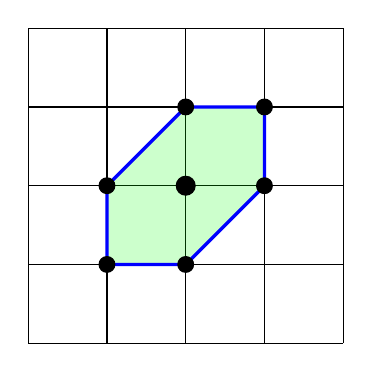
\begin{tikzpicture}
  \draw (0, 0) grid (4, 4);  
\draw [very thick, color=blue, fill=green, fill opacity=0.2]
(1,1) -- (2,1) -- (3,2) -- (3,3) -- (2,3) -- (1,2) -- cycle;
\draw [fill=black]  (1, 1) circle (0.1);
\draw [fill=black]  (2, 1) circle (0.1);
\draw [fill=black]  (3, 2) circle (0.1);
\draw [fill=black]  (3, 3) circle (0.1);s
\draw [fill=black]  (2, 3) circle (0.1);
\draw [fill=black]  (1, 2) circle (0.1);
\draw [fill=black]  (2, 2) circle (0.12);
\end{tikzpicture}
\caption{A hexagon.}
\label{fig:hexagon}
\end{figure}

By starring $E_6$ with a vertex, we get a triangulation of the disk. Denote by $\nabla$, the hexagon in  \cref{fig:hexagon}. By Theorem 8.3 and Corollary 8.9 in \cite{sturmfels}, there is a one-one correspondence between unimodular regular triangulations of $\nabla$ and the square-free initial ideals of the toric ideal of $\P(\nabla)$. 

This means that $E_6 \ast \{ pt \}$ smooths to the del Pezzo surface of degree $6$, and also that $\P(E_6)$ smooths to an anticanonical section of $\dP6$. 

\todo{Talk about the join of two del pezzos}

$X_0$.

\section[Smoothings of X0]{Smoothings of $X_0$}

We will exploit the fact that the cone over $\dP6$ have two smoothings two produce two smoothings of $X_0$.